% NOTES:
% enum slide
% difference between := and =
% link and plink pic
% filter pic
% examples of running chisel

\documentclass[xcolor=pdflatex,dvipsnames,table]{beamer}
\usepackage{epsfig,graphicx}
\usepackage{palatino}
\usepackage{fancybox}
\usepackage{relsize}
\usepackage[procnames]{listings}

% "define" Scala
\usepackage[T1]{fontenc}  
\usepackage[scaled=0.82]{beramono}  
\usepackage{microtype} 

\sbox0{\small\ttfamily A}
\edef\mybasewidth{\the\wd0 }

\lstdefinelanguage{scala}{
  morekeywords={abstract,case,catch,class,def,%
    do,else,extends,false,final,finally,%
    for,if,implicit,import,match,mixin,%
    new,null,object,override,package,%
    private,protected,requires,return,sealed,%
    super,this,throw,trait,true,try,%
    type,val,var,while,with,yield},
  sensitive=true,
  morecomment=[l]{//},
  morecomment=[n]{/*}{*/},
  morestring=[b]",
  morestring=[b]',
  morestring=[b]"""
}

\usepackage{color}
\definecolor{dkgreen}{rgb}{0,0.6,0}
\definecolor{gray}{rgb}{0.5,0.5,0.5}
\definecolor{mauve}{rgb}{0.58,0,0.82}

% Default settings for code listings
\lstset{frame=tb,
  language=scala,
  aboveskip=3mm,
  belowskip=3mm,
  showstringspaces=false,
  columns=fixed, % basewidth=\mybasewidth,
  basicstyle={\small\ttfamily},
  numbers=none,
  numberstyle=\footnotesize\color{gray},
  % identifierstyle=\color{red},
  keywordstyle=\color{blue},
  commentstyle=\color{dkgreen},
  stringstyle=\color{mauve},
  frame=single,
  breaklines=true,
  breakatwhitespace=true,
  procnamekeys={def, val, var, class, trait, object, extends},
  procnamestyle=\ttfamily\color{red},
  tabsize=2
}

\lstnewenvironment{scala}
{\lstset{language=scala}}
{}
\lstnewenvironment{cpp}
{\lstset{language=C++}}
{}
\lstnewenvironment{bash}
{\lstset{language=bash}}
{}
\lstnewenvironment{verilog}
{\lstset{language=verilog}}
{}


\lstset{basicstyle={\footnotesize\ttfamily}}

\usetheme[height=8mm]{Rochester}
\setbeamersize{text margin left=3mm} 
\setbeamersize{text margin right=3mm} 
\setbeamertemplate{navigation symbols}{}

\definecolor{Cobalt}{rgb}{0.25,0.125,0.70}
\definecolor{RedOrange}{rgb}{0.8,0.25,0.0}
% \definecolor{RedOrange}{rgb}{0.8,0.775,0.25}
\def\frametitledefaultcolor{Cobalt}
\def\frametitleproblemcolor{RedOrange}

\lstset{basicstyle={\footnotesize\ttfamily}}

\setbeamertemplate{frametitle}
{
\vskip-7mm
\textbf{\insertframetitle}\hfill\insertframenumber
}
\setbeamercolor{frametitle}{bg=\frametitledefaultcolor}

\newenvironment{sample}{\VerbatimEnvironment\begin{footnotesize}\begin{semiverbatim}}{\end{semiverbatim}\end{footnotesize}}

\newenvironment{FramedSemiVerb}%
{\begin{Sbox}\begin{minipage}{.94\textwidth}\begin{semiverbatim}}%
{\end{semiverbatim}\end{minipage}\end{Sbox}
\setlength{\fboxsep}{8pt}\fbox{\TheSbox}}

\newenvironment{FramedVerb}%
{\VerbatimEnvironment
\begin{Sbox}\begin{minipage}{.94\textwidth}\begin{Verbatim}}%
{\end{Verbatim}\end{minipage}\end{Sbox}
\setlength{\fboxsep}{8pt}\fbox{\TheSbox}}

% \newenvironment{sample}{\VerbatimEnvironment\begin{footnotesize}\begin{Verbatim}}{\end{Verbatim}\end{footnotesize}}
\newcommand{\code}[1]{\begin{footnotesize}{\tt #1}\end{footnotesize}}
\newcommand{\comment}[1]{{\color{Green}\it\smaller #1}}


\title{Chisel @ CS250 -- Part I -- Lecture 02}
\author{Jonathan Bachrach}
\date{\today}
\institute[UC Berkeley]{EECS UC Berkeley}

\begin{document}

\begin{frame}
\titlepage
\end{frame}
\addtocounter{framenumber}{-1}

% \begin{frame}[fragile]{tutorial.scala}
% \begin{scala}
% package Tutorial {
% 
% import Chisel._
% 
% object Tutorial {
%   def main(args: Array[String]): Unit = { 
%     val tut_args = args.slice(1, args.length) ++ 
%       Array("--targetDir", "../emulator", "--genHarness")
%     args(0) match {
%       case "gcd" => 
%         chiselMain(tut_args, () => new GCD())
%       ...
%     }
%   }
% }
% 
% }
% \end{scala}
% \end{frame}

\begin{frame}
\frametitle{Standard Design Methodology}
\begin{center}
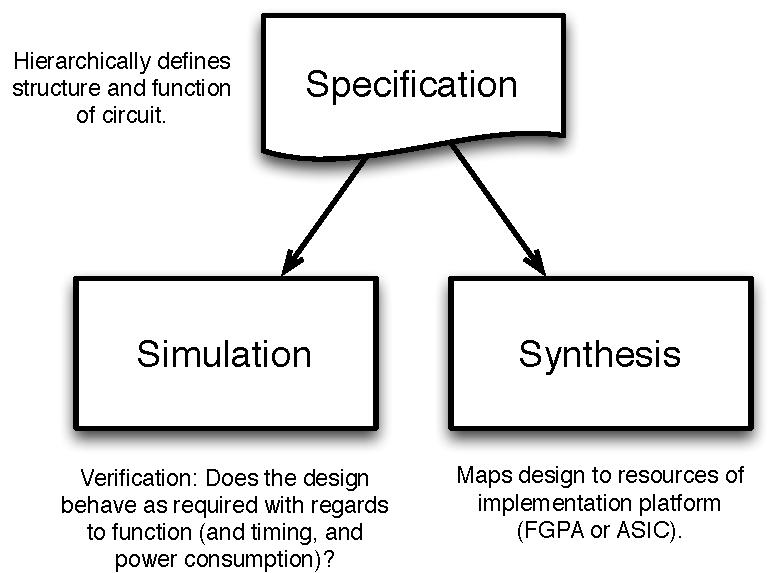
\includegraphics[height=0.9\textheight]{figs/design.pdf}
\end{center}
\end{frame}

\begin{frame}
\frametitle{Design Entry}
\begin{columns}[c]
\column{0.5\textwidth}
\begin{itemize}
\item Design circuits graphically
\item Used commonly until approximately 2002
\item Schematics are intuitive
\item Labor intensive to produce (especially readable ones).
\item Requires a special editor tool
\item Unless hierarchy is carefully designed, schematics can be confusing and difficult to follow on large designs
\end{itemize}
\column{0.5\textwidth}
\begin{center}
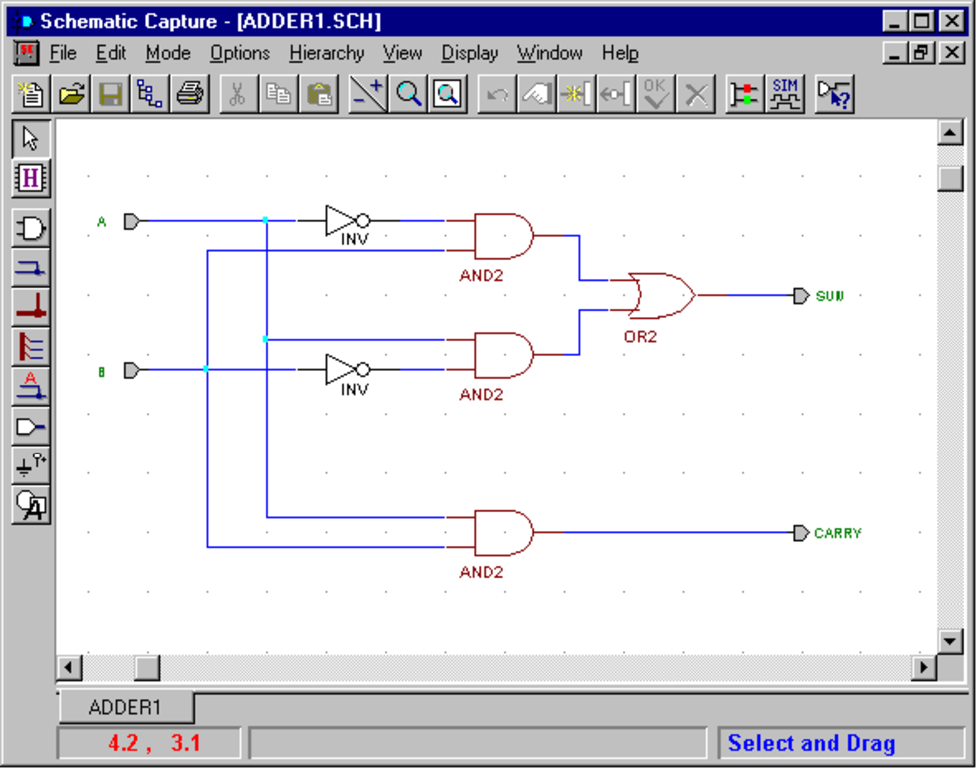
\includegraphics[height=0.4\textheight]{figs/schematic-capture.pdf}
\end{center}
\end{columns}
\end{frame}

\begin{frame}[fragile]
\frametitle{Hardware Description Languages}
\begin{columns}[c]
\column{0.45\textwidth}
\textbf{Structural Description}: connections of components with a nearly one-to-one correspondence to schematic diagram.
\begin{scala}
Decoder(output x0,x1,x2,x3; 
        input a,b) {
  wire abar, bbar;
  inv(bbar, b);
  inv(abar, a);
  and(x0, abar, bbar);
  and(x1, abar, b   );
  and(x2, a,    bbar);
  and(x3, a,    b   );
} 
\end{scala}
\column{0.45\textwidth}
\textbf{Behavioral Description}: use high-level constructs (similar to convential programming) to describe the circuit function.
\begin{scala}
Decoder(output x0,x1,x2,x3; 
        input a,b) {
  case [a b]
    00: [x0 x1 x2 x3] = 0x1;
    01: [x0 x1 x2 x3] = 0x2;
    10: [x0 x1 x2 x3] = 0x4;
    11: [x0 x1 x2 x3] = 0x8;
  endcase;
}
\end{scala}
\end{columns}
\end{frame}

\begin{frame}

\frametitle{Verilog Issues}
\begin{itemize}
\item Originally invented for simulation
\item Many constructs don't synthesize: ex: deassign, timing constructs
\item Others lead to mysterious results: for-loops
\item Difficult to understand synthesis implications of procedural assignments (always blocks), and blocking versus non-blocking assignments
\item In common use, most users ignore much of the language and stick to a very strict style
\item Very weak meta programming support for creating circuit generators
\item Various hacks around this over the years, ex: embedded TCL scripting
\item VHDL has much the same issues
\end{itemize}

\end{frame}

\begin{frame}

\frametitle{Chisel}

\textbf{Constructing Hardware In Scala Embedded Language}
\begin{itemize}
\item Embed a hardware-description language in Scala, using Scala's extension facilities
\item Chisel is just a set of class definitions in Scala and when you write a Chisel program you are actually writing a Scala program
\item A hardware module is just a data structure in Scala
\item Clean simple set of design construction primitives for RTL design
\item Full power of Scala for writing hardware generators
\item Different output routines can generate different types of output (C, FPGA-Verilog, ASIC-Verilog) from same hardware representation
\item Can be extended above with domain specific languages (such as declarative cache coherence specifications)
\item Can be extended below with new backends (such as quantum)
\item Open source with lots of libraries
\item Only 5200 lines of code in current version!
\end{itemize}

\end{frame}

\begin{frame}
\frametitle{Chisel Workflow}
\begin{center}
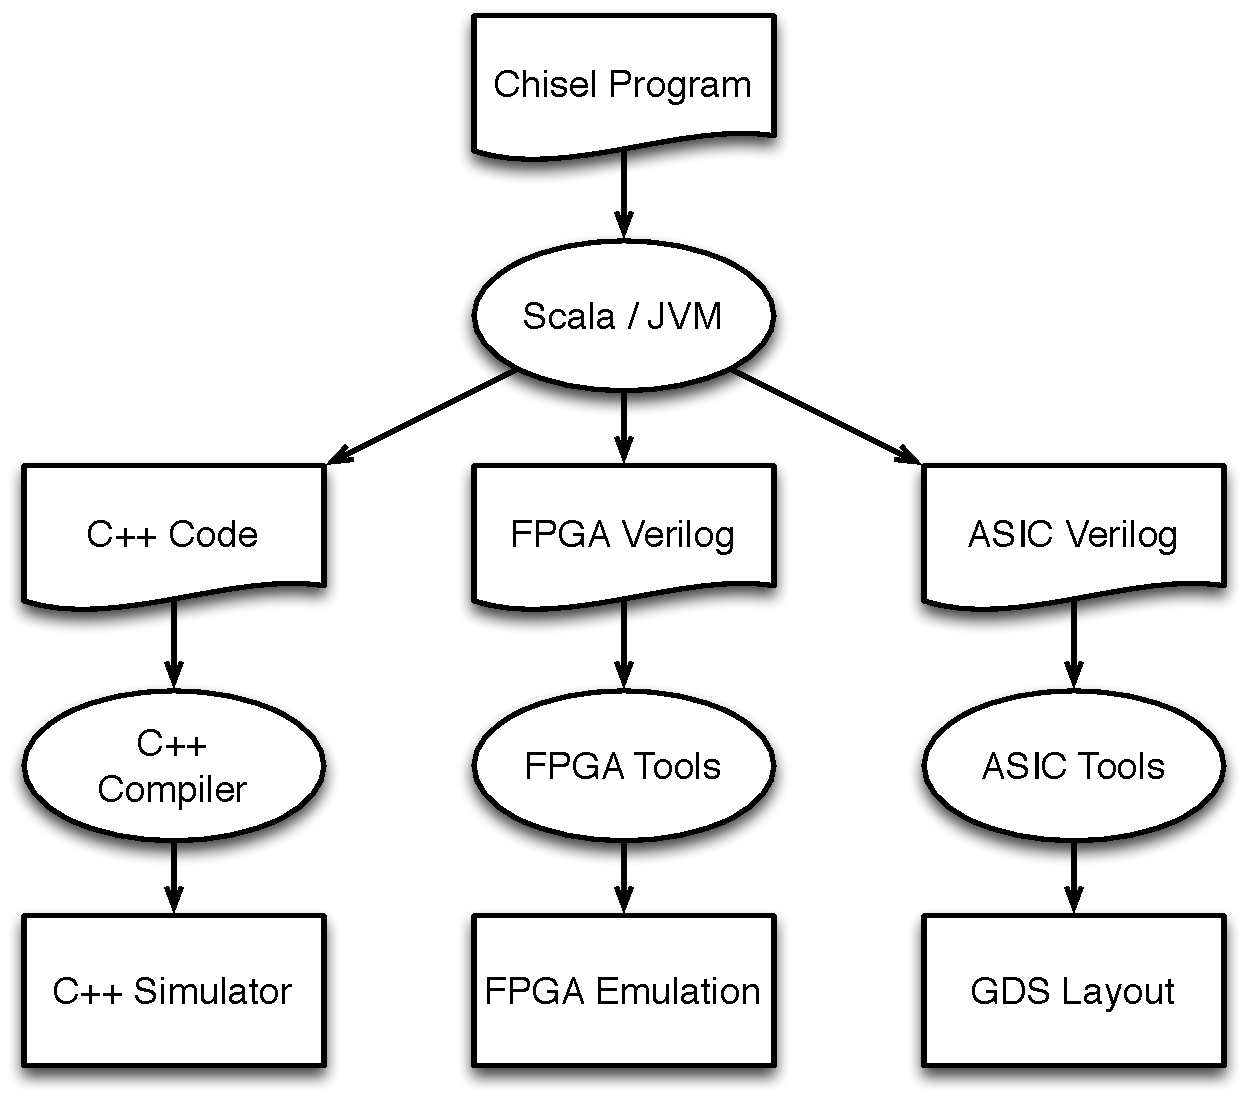
\includegraphics[height=0.9\textheight]{figs/workflow.pdf}
\end{center}

\end{frame}

\begin{frame}[fragile]
\frametitle{The Scala Programming Language}

\begin{columns}[c]

\column{0.75\textwidth}

\begin{itemize}
\item Compiled to JVM
\begin{itemize}
\item Good performance
\item Great Java interoperability
\item Mature debugging, execution environments
\end{itemize}
\item Object Oriented
\begin{itemize}
\item Factory Objects, Classes
\item Traits, overloading etc
\end{itemize}
\item Functional
\begin{itemize}
\item Higher order functions
\item Anonymous functions
\item Currying etc
\end{itemize}
\item Extensible
\begin{itemize}
\item Domain Specific Languages (DSLs)
\end{itemize}
\end{itemize}

\column{0.25\textwidth}

\begin{center}
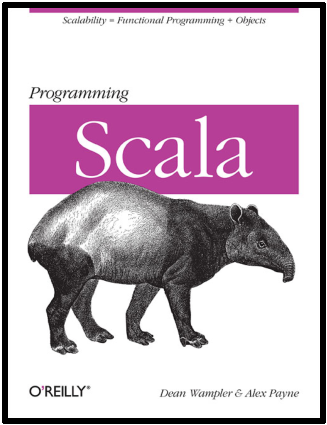
\includegraphics[height=0.4\textheight]{../bootcamp/figs/programming-scala.pdf} \\
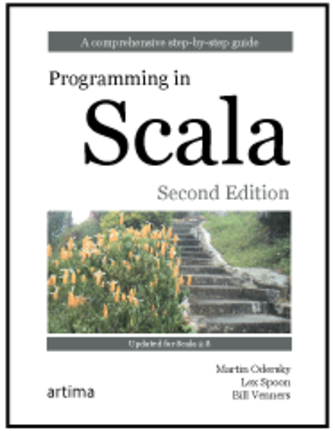
\includegraphics[height=0.4\textheight]{../bootcamp/figs/programming-in-scala.pdf}
\end{center}

\end{columns}
\end{frame}

\begin{frame}[fragile]{Scala Collections}
\begin{scala}
// Array's
val tbl = new Array[Int](256)
tbl(0) = 32
val y = tbl(0)
val n = tbl.length

// ArrayBuffer's
val buf = new ArrayBuffer[Int]()
buf += 12
val z = buf(0)
val l = buf.length

// List's
val els = List(1, 2, 3)
val a :: b :: c :: Nil = els
val m = els.length
\end{scala}
\end{frame}

\begin{frame}[fragile]{Scala Iteration}
\begin{scala}
val tbl = new Array[Int](256)

// loop over all indices
for (i <- 0 until tbl.length)
  tbl(i) = i

// loop of each sequence element
for (e <- tbl)
  tbl(i) += e

// nested loop
for (i <- 0 until 16; j <- 0 until 16)
  tbl(j*16 + i) = i

// create second table with doubled elements
val tbl2 = for (i <- 0 until 16) yield tbl(i)*2
\end{scala}
\end{frame}

\begin{frame}[fragile]{Scala Functional}
\begin{scala}
// simple scaling function, e.g., x2(3) => 6
def x2 (x: Int) = 2 * x
\end{scala}

\begin{scala}
// produce list of 2 * elements, e.g., x2list(List(1, 2, 3)) => List(2, 4, 6)
def x2list (xs: List[Int]) = xs.map(x2)
\end{scala}

\begin{scala}
// simple addition function, e.g., add(1, 2) => 3
def add (x: Int, y: Int) = x + y
\end{scala}

\begin{scala}
// sum all elements using pairwise reduction, e.g., sum(List(1, 2, 3)) => 6
def sum (xs: List[Int]) = xs.foldLeft(0)(add)
\end{scala}
\end{frame}

\begin{frame}[fragile]{Scala Object Oriented}

\begin{scala}
object Blimp {
  var numBlimps = 0
  def apply(r: Double) = {
    numBlimps += 1
    new Blimp(r)
  }
}

Blimp.numBlimps
Blimp(10.0)

class Blimp(r: Double) {
  val rad = r
  println("Another Blimp")
}

class Zep(r: Double) extends Blimp(r)
\end{scala}

\end{frame}

\begin{frame}[fragile]{Scala Console}
\begin{scala}
> scala
scala> 1 + 2
=> 3
scala> def f (x: Int) = 2 * x
=> (Int) => Int
scala> f(4)
=> 8
\end{scala}
\end{frame}

% \begin{frame}[fragile]
% \frametitle{Example}
% \begin{columns}
% 
% \column{0.45\textwidth}
% 
% \begin{footnotesize}
% \begin{scala}
% class GCD extends Module {
%   val io = new Bundle {
%     val a     = UInt(INPUT, 16)
%     val b     = UInt(INPUT, 16)
%     val z     = UInt(OUTPUT, 16)
%     val valid = Bool(OUTPUT) }
%   val x = Reg(reset = io.a)
%   val y = Reg(reset = io.b)
%   when (x > y) {
%     x := x - y
%   } .otherwise {
%     y := y - x
%   }
%   io.z     := x
%   io.valid := y === UInt(0)
% }
% \end{scala}
% \end{footnotesize}
% 
% \column{0.45\textwidth}
% 
% \begin{center}
% 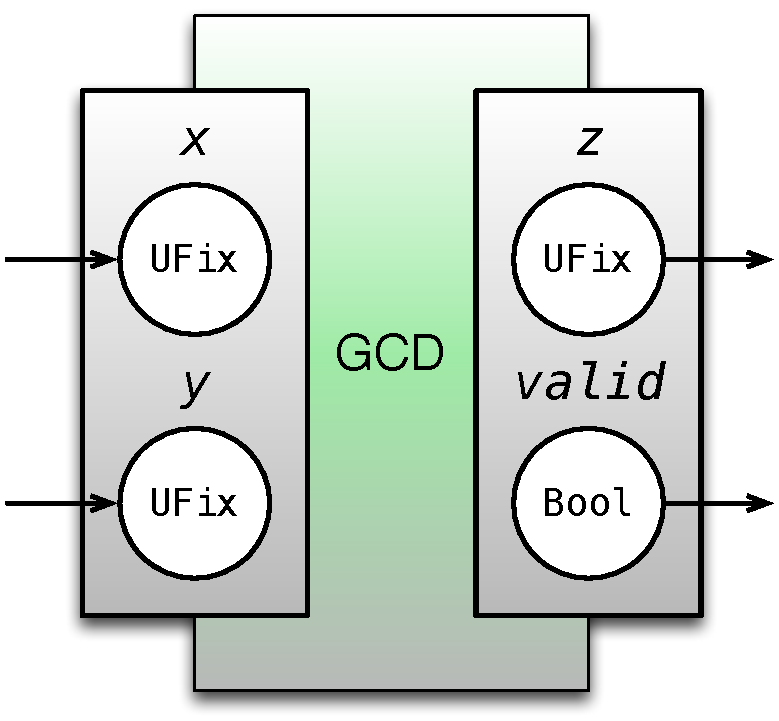
\includegraphics[width=0.9\textwidth]{figs/gcd.pdf} 
% \end{center}
% 
% \end{columns}
% \end{frame}

\begin{frame}[fragile]
\frametitle{Chisel Example}
\begin{columns}

\column{0.40\textwidth}

\begin{footnotesize}
\begin{scala}
class Mux2 extends Module {
  val io = new Bundle{
    val sel = UInt(INPUT, 1)
    val in0 = UInt(INPUT, 1)
    val in1 = UInt(INPUT, 1)
    val out = UInt(OUTPUT, 1)
  }
  io.out := (io.sel & io.in1) | 
            (~io.sel & io.in0)
}
\end{scala}
\end{footnotesize}

\column{0.50\textwidth}

\begin{center}
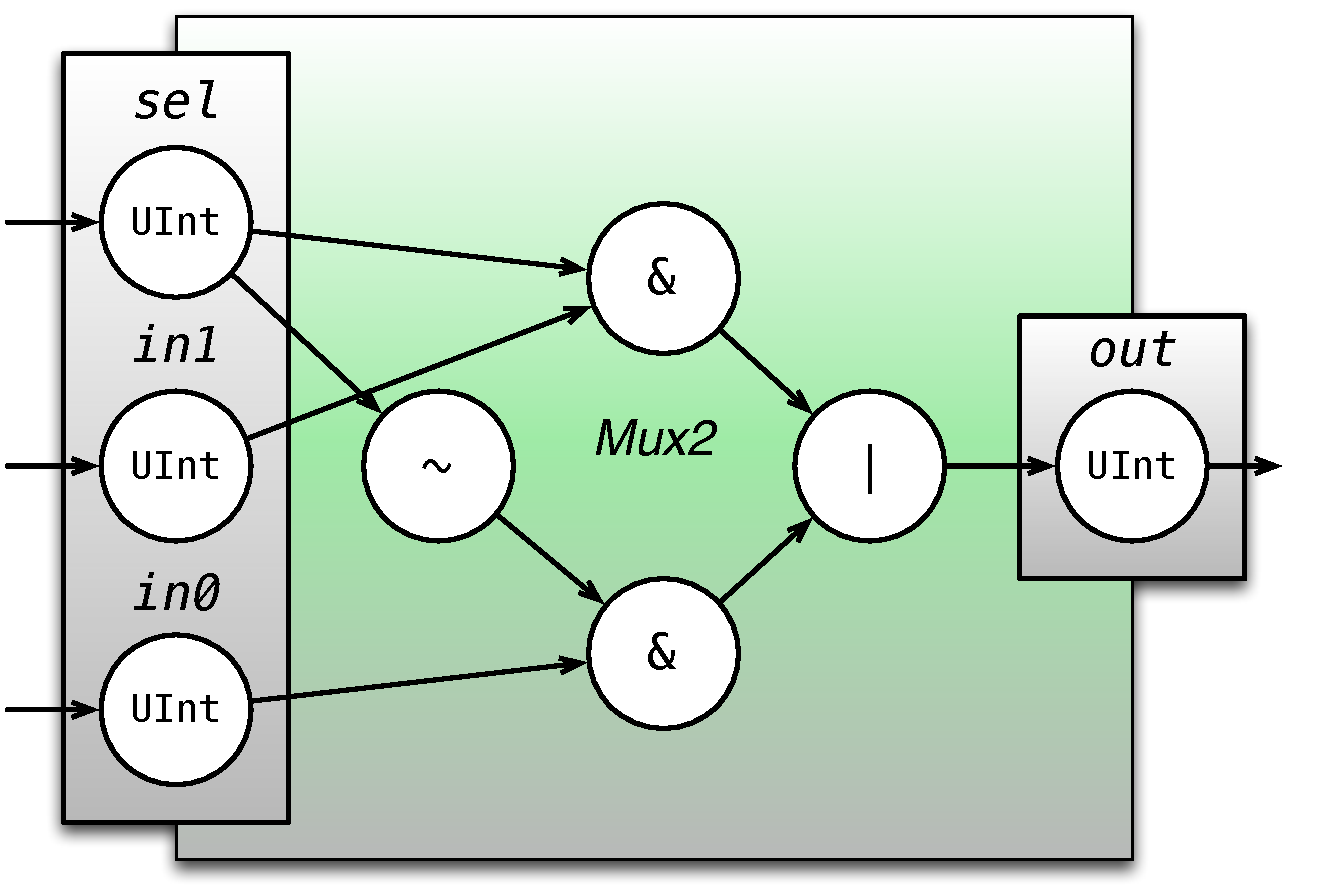
\includegraphics[width=0.9\textwidth]{figs/mux2-component.pdf} 
\end{center}

\end{columns}
\end{frame}

% \begin{frame}[fragile]{Scala Console}
% \begin{FramedVerb}
% \end{FramedVerb}
% \end{frame}

\begin{frame}[fragile]{Literals}
\begin{scala}
UInt(1)       // decimal 1-bit literal from Scala Int. 
UInt("ha")    // hexadecimal 4-bit literal from string.
UInt("o12")   // octal 4-bit literal from string. 
UInt("b1010") // binary 4-bit literal from string.

SInt(5)       // signed decimal 4-bit literal from Scala Int.
SInt(-8)      // negative decimal 4-bit literal from Scala Int.
UInt(5)       // unsigned decimal 3-bit literal from Scala Int.

Bool(true)    // Bool literals from Scala literals.
Bool(false)
\end{scala}
\end{frame}
 
\begin{frame}[fragile]{Literals}
\begin{scala}
UInt("h_dead_beef") // 32-bit literal of type UInt.
UInt(1)             // decimal 1-bit literal from Scala Int.
UInt("ha", 8)       // hexadecimal 8-bit literal of type UInt.
UInt("o12", 6)      // octal 6-bit literal of type UInt.
UInt("b1010", 12)   // binary 12-bit literal of type UInt.

SInt(5, 7)          // signed decimal 7-bit literal of type SInt.
UInt(5, 8)          // unsigned decimal 8-bit literal of type UInt.
\end{scala}
\end{frame}

\begin{frame}[fragile]{Literal Node Construction}

\begin{scala}
UInt(1)
\end{scala}

\begin{center}
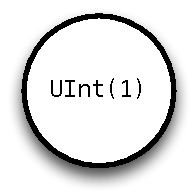
\includegraphics[height=0.7\textheight]{figs/ufix.pdf} 
\end{center}

\end{frame}


\begin{frame}[fragile]{Algebraic Construction}

\begin{scala}
UInt(1) + UInt(2)
\end{scala}

\begin{center}
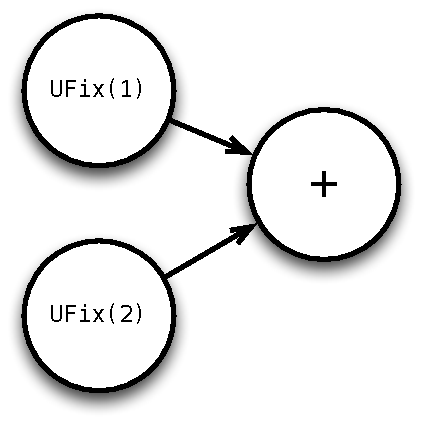
\includegraphics[height=0.7\textheight]{figs/add.pdf} 
\end{center}

\end{frame}


\begin{frame}[fragile]{Combinational Circuits}

\begin{scala}
(sel & in1) | (~sel & in0)
\end{scala}

\begin{center}
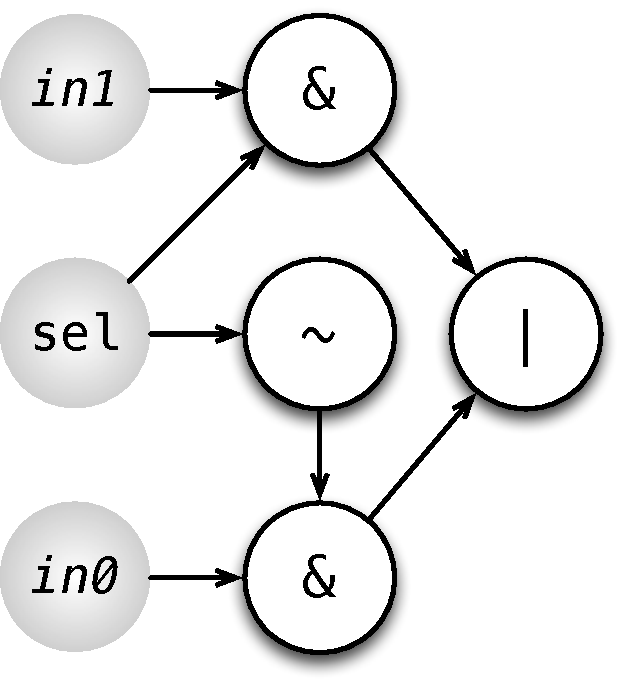
\includegraphics[height=0.7\textheight]{figs/mux2-circuit.pdf} 
\end{center}

\end{frame}

\begin{frame}[fragile]{Fan Out}

\begin{scala}
val sel = a | b
val out = (sel & in1) | (~sel & in0)
\end{scala}

\begin{center}
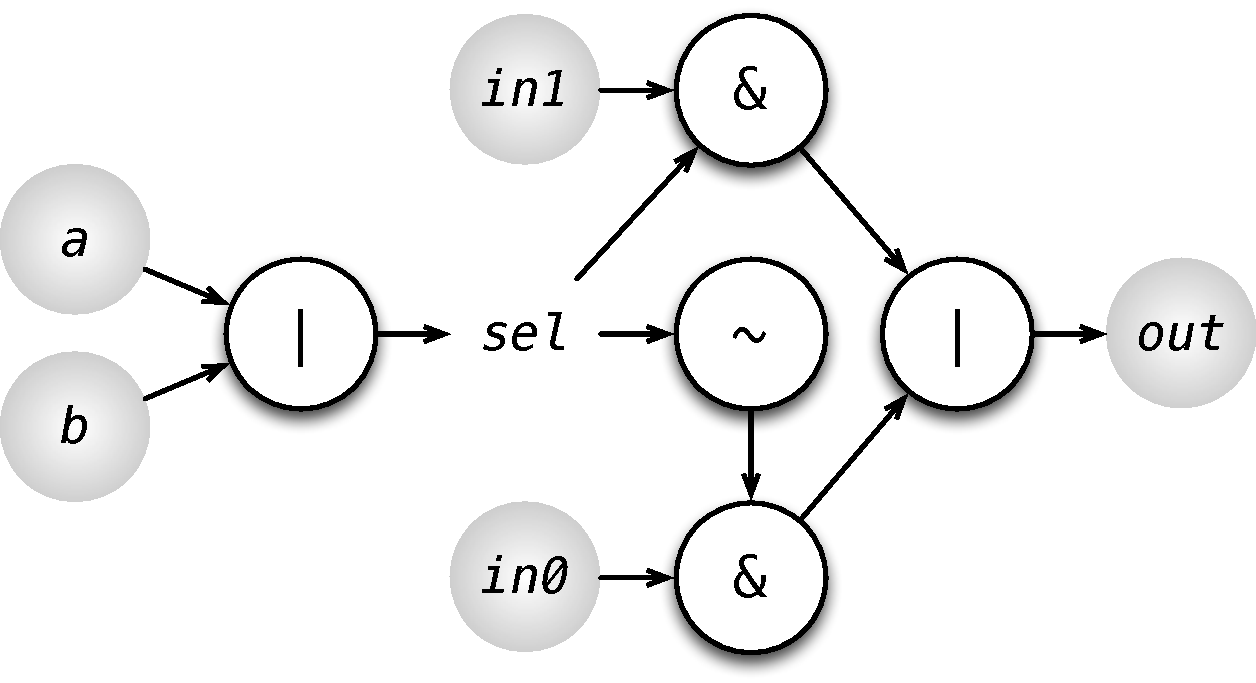
\includegraphics[height=0.7\textheight]{figs/mux2-named-sel.pdf} 
\end{center}

\end{frame}

\begin{frame}[fragile]{Wires}

\begin{scala}
val sel = UInt()
val out = (sel & in1) | (~sel & in0)
sel := a | b
\end{scala}

\begin{center}
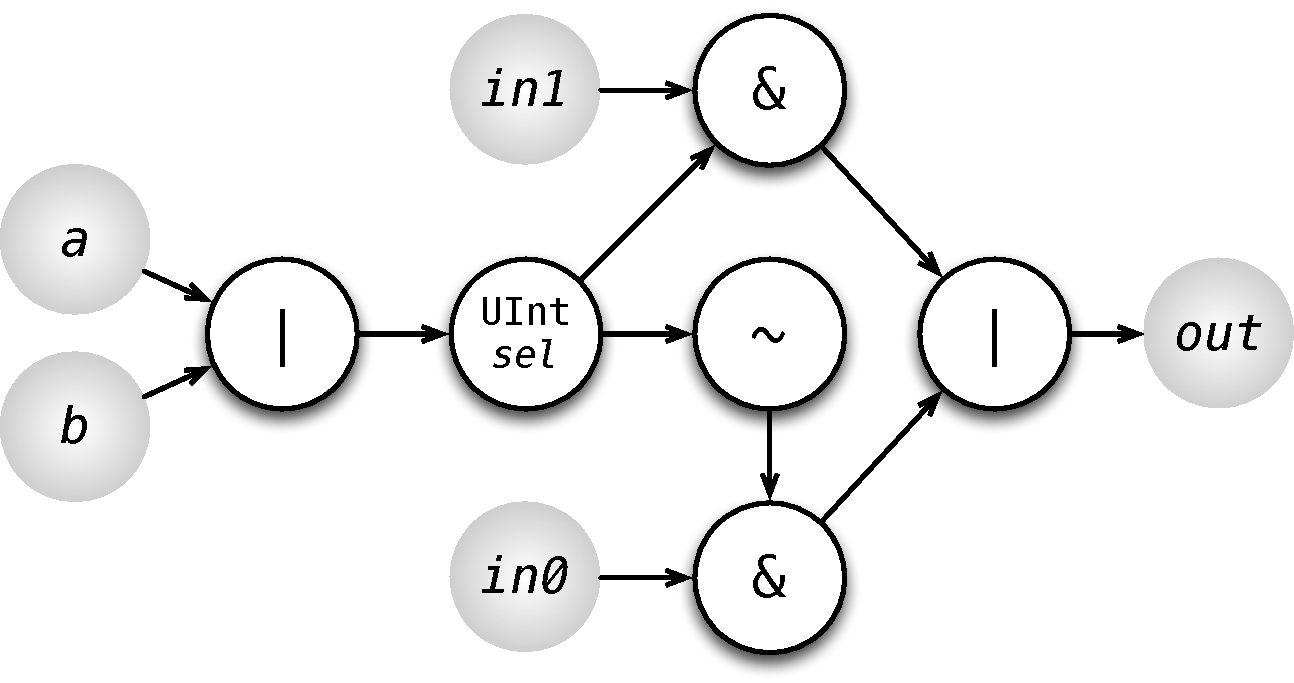
\includegraphics[width=0.9\textwidth]{figs/mux2-forward-sel.pdf} 
\end{center}

\end{frame}

\begin{frame}[fragile]{Bitwise operators}
\textbf{Valid on UInt, SInt, Bool.}
\begin{scala}
// Bitwise-NOT
val invertedX = ~x                      
// Bitwise-AND 
val hiBits    = x & UInt("h_ffff_0000") 
// Bitwise-OR
val flagsOut  = flagsIn | overflow      
// Bitwise-XOR
val flagsOut  = flagsIn ^ toggle        
\end{scala}
\end{frame}

\begin{frame}[fragile]{Bitwise reductions}
\textbf{Valid on UInt and SInt.  Returns Bool.}
\begin{scala}
// AND-reduction 
val allSet = andR(x)  
// OR-reduction
val anySet = orR(x)   
// XOR-reduction 
val parity = xorR(x)  
\end{scala}
\noindent
where reduction applies the operation to all the bits.
\end{frame}

\begin{frame}[fragile]{Equality comparison}
\textbf{Valid on UInt, SInt, and Bool. Returns Bool.}
\begin{scala}
// Equality
val equ = x === y 
// Inequality 
val neq = x != y   
\end{scala}
\noindent
where \verb+===+ is used instead of \verb+==+ to avoid collision with Scala.
\end{frame}

\begin{frame}[fragile]{Shifts}
\textbf{Valid on SInt and UInt.}
\begin{scala}
// Logical left shift.
val twoToTheX = SInt(1) << x   
// Right shift (logical on UInt & UInt, arithmetic on SInt).
val hiBits    = x >> UInt(16) 
\end{scala}
\noindent
where logical is a raw shift and arithmetic performs top bit sign extension.
\end{frame}

\begin{frame}[fragile]{Bitfield manipulation}
\textbf{Valid on SInt, UInt, and Bool.}
\begin{scala}
// Extract single bit, LSB has index 0.
val xLSB       = x(0)                
// Extract bit field  from end to start bit pos. 
val xTopNibble = x(15,12)            
// Replicate a bit string multiple times.
val usDebt     = Fill(3, UInt("hA")) 
// Concatenates bit fields, w/ first arg on left
val float      = Cat(sgn,exp,man)    
\end{scala}
\end{frame}

\begin{frame}[fragile]{Logical Operations}
\textbf{Valid on Bools. }
\begin{scala}
// Logical NOT. 
val sleep = !busy                     
// Logical AND.
val hit   = tagMatch && valid         
// Logical OR.
val stall = src1busy || src2busy      
// Two-input mux where sel is a Bool.  
val out   = Mux(sel, inTrue, inFalse) 
\end{scala}
\end{frame}

\begin{frame}[fragile]{Arithmetic operations}
\textbf{Valid on Nums: SInt and UInt. }
\begin{scala}
// Addition. 
val sum  = a + b  
// Subtraction.
val diff = a - b  
// Multiplication. 
val prod = a * b  
// Division.
val div  = a / b  
// Modulus
val mod  = a % b  
\end{scala}
\noindent
where \verb+SInt+ is a signed fixed-point number represented in two's complement and \verb+UInt+ is an unsigned fixed-point number. 
\end{frame}

\begin{frame}[fragile]{Arithmetic comparisons}
\textbf{Valid on Nums: SInt and UInt. Returns Bool.}
\begin{scala}
// Greater than.
val gt  = a > b   
// Greater than or equal.
val gte = a >= b  
// Less than.
val lt  = a < b   
// Less than or equal.
val lte = a <= b  
\end{scala}
\end{frame}

\begin{frame}[fragile]{Bitwidth Inference}
\begin{center}
\begin{tabular}{ll}
{\bf operation} & {\bf bit width} \\ 
\verb|z = x + y| & \verb+wz = max(wx, wy)+ \\
\verb+z = x - y+ & \verb+wz = max(wx, wy)+\\
\verb+z = x & y+ & \verb+wz = min(wx, wy)+ \\
\verb+z = x | y+ & \verb+wz = max(wx, wy)+ \\
\verb+z = Mux(c, x, y)+ & \verb+wz = max(wx, wy)+ \\
\verb+z = w * y+ & \verb!wz = wx + wy! \\
\verb+z = x << n+ & \verb!wz = wx + maxNum(n)! \\
\verb+z = x >> n+ & \verb+wz = wx - minNum(n)+ \\
\verb+z = Cat(x, y)+ & \verb!wz = wx + wy! \\
\verb+z = Fill(n, x)+ & \verb+wz = wx * maxNum(n)+ \\
% \verb+z = x < y+ & \verb+<= > >= && || != ===+ & \verb+wz = 1+ \\
\end{tabular}
\end{center}
\end{frame}

% \begin{frame}[fragile]{Node Class Hierarchy}
% 
% \begin{center}
% 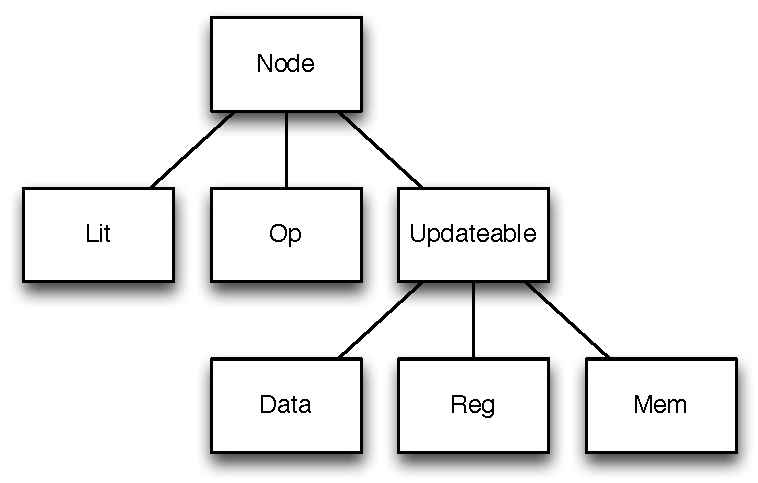
\includegraphics[height=0.9\textheight]{../manual/figs/node-hierarchy.pdf}
% \end{center}
% 
% \end{frame}

\begin{frame}[fragile]{Functional Abstraction}
\begin{scala}
def mux2 (sel: UInt, in0: UInt, in1: UInt) = 
  (sel & in1) | (~sel & in0)

val out = mux2(k,a,b)
\end{scala}
\begin{center}
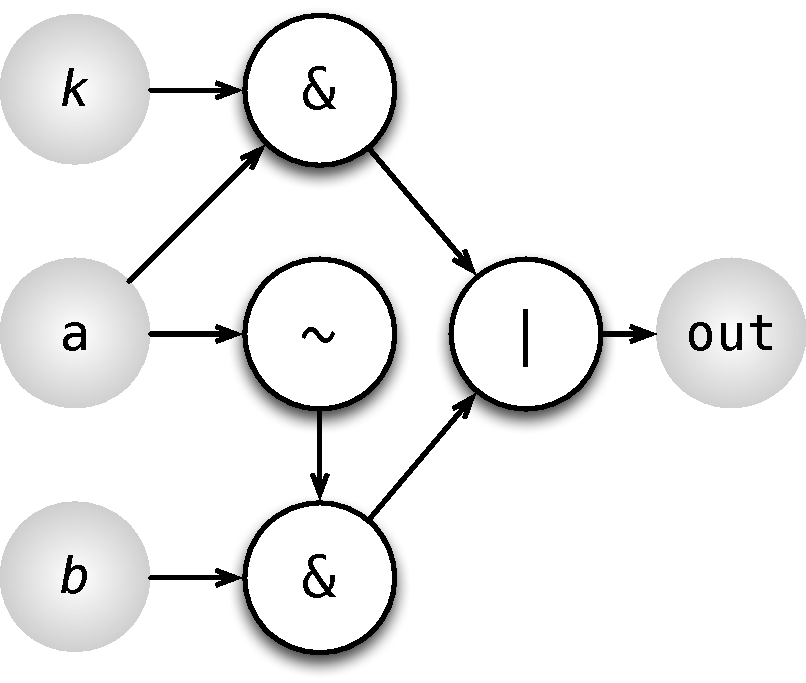
\includegraphics[height=0.7\textheight]{figs/mux2-function.pdf} 
\end{center}
\end{frame}

\begin{frame}[fragile]{Bundles}

\begin{columns}
\column{0.55\textwidth}
\begin{scala}
class MyFloat extends Bundle {
  val sign        = Bool()
  val exponent    = UInt(width = 8)
  val significand = UInt(width = 23)
}

val x  = new MyFloat()
val xs = x.sign
\end{scala}

\column{0.35\textwidth}

\begin{center}
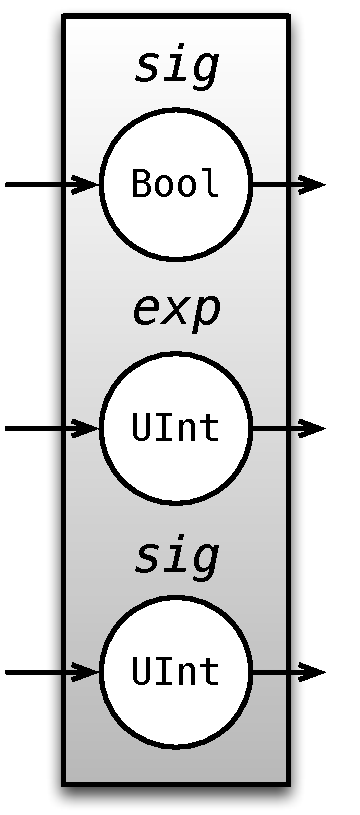
\includegraphics[height=0.9\textheight]{figs/myfloat.pdf} 
\end{center}

\end{columns}
\end{frame}

\begin{frame}[fragile]{Vecs}
\begin{columns}
\column{0.55\textwidth}

\begin{scala}
// Vector of 3 23-bit signed integers.
val myVec = Vec.fill(3) { SInt(width = 23) } 
\end{scala}

\begin{itemize}
\item can be used as Scala sequences
\item can also be nested into Chisel Bundles
\end{itemize}

\column{0.35\textwidth}

\begin{center}
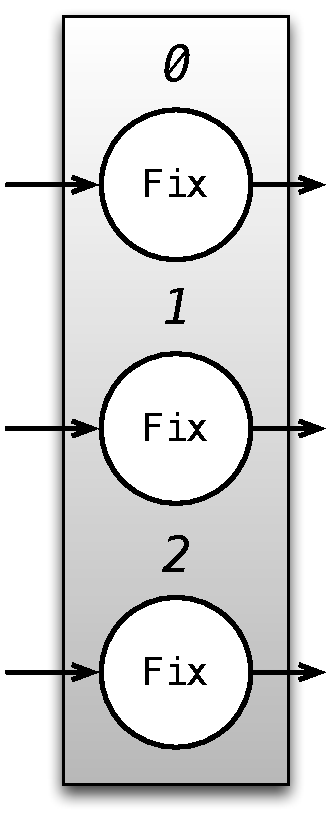
\includegraphics[height=0.9\textheight]{figs/vec-3-fix.pdf} 
\end{center}

\end{columns}
\end{frame}

\begin{frame}[fragile]{Static Vec Element Access}
\begin{scala}
val myVec = Vec.fill(3) { SInt(width = 23) } 

// Connect to one vector element chosen at elaboration time.
val fix0  = myVec(0)
val fix1  = myVec(1)
fix1     := data1 
myVec(2) := data2
\end{scala}

\begin{center}
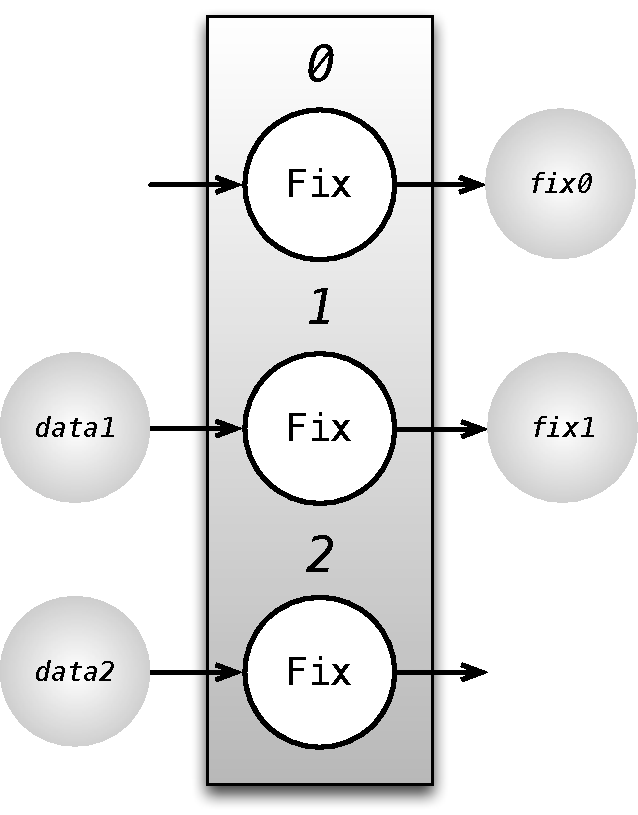
\includegraphics[height=0.5\textheight]{figs/vec-3-static.pdf} 
\end{center}
\end{frame}

\begin{frame}[fragile]{Dynamic Vec Element Access}
\begin{scala}
val myVec = Vec.fill(3) { SInt(width = 23) } 

// Connect to one vector element chosen at runtime.
val out0      = myVec(addr0)
val out1      = myVec(addr1)
myVec(addr2) := data2
\end{scala}

\begin{center}
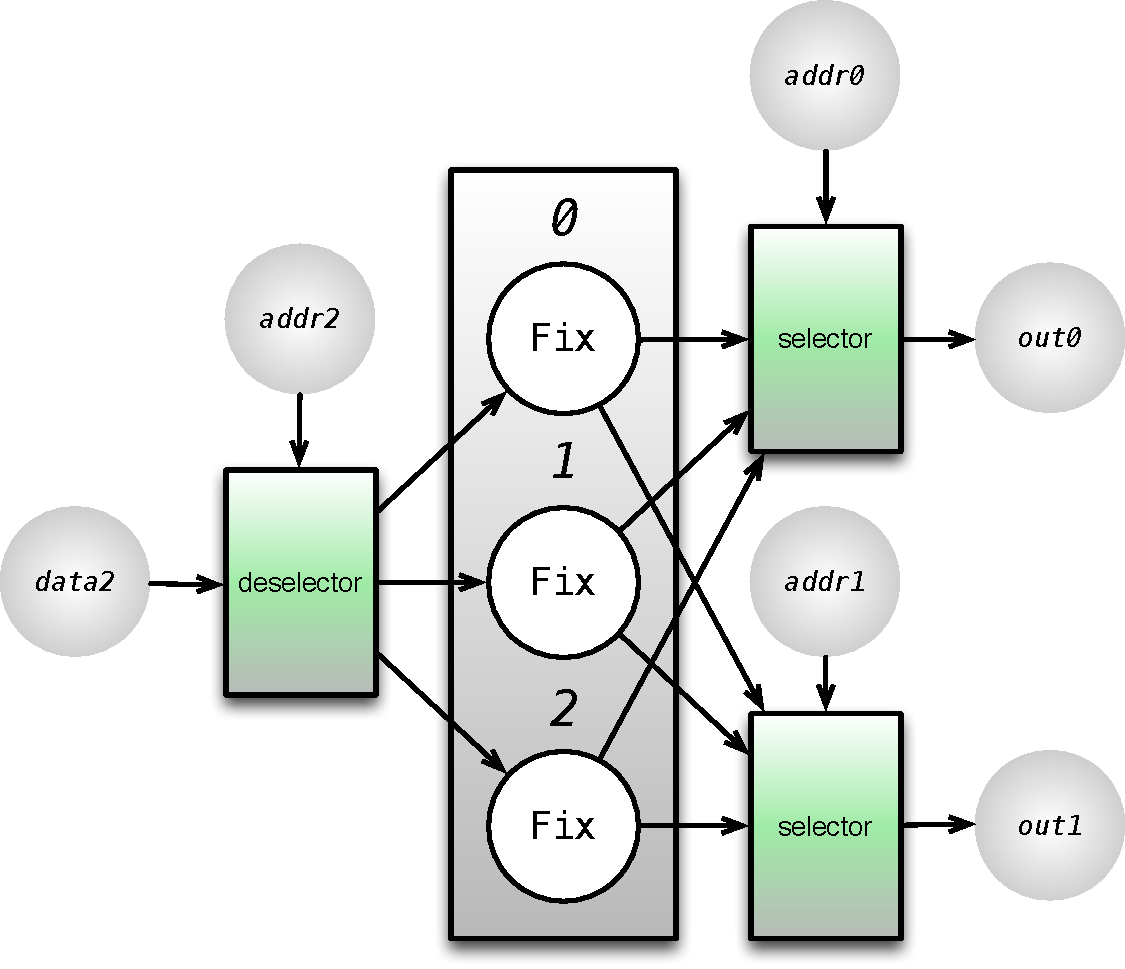
\includegraphics[height=0.6\textheight]{figs/vec-3-dynamic.pdf} 
\end{center}
\end{frame}

\begin{frame}[fragile]{Ports}

\begin{columns}
\column{0.55\textwidth}

\textbf{Data object with directions assigned to its members}

\begin{scala}
class Decoupled extends Bundle {
  val data  = UInt(INPUT, 32)
  val valid = Bool(OUTPUT)
  val ready = Bool(INPUT)
}
\end{scala}

\textbf{Direction assigned at instantiation time}

\begin{scala}
class ScaleIO extends Bundle {
  val in    = new MyFloat().asInput
  val scale = new MyFloat().asInput
  val out   = new MyFloat().asOutput
}
\end{scala}

\column{0.35\textwidth}

\begin{center}
\includegraphics[height=0.9\textheight]{figs/fifoio.pdf} 
\end{center}

\end{columns}

\end{frame}

\begin{frame}[fragile]{Module}

\begin{columns}
\column{0.45\textwidth}

\begin{itemize}
\item inherits from \verb+Module+,
\item contains an interface stored in a port field named \verb+io+, and
\item wires together subcircuits in its constructor.
\end{itemize}

\begin{scala}
class Mux2 extends Module {
  val io = new Bundle{
    val sel = UInt(INPUT, 1)
    val in0 = UInt(INPUT, 1)
    val in1 = UInt(INPUT, 1)
    val out = UInt(OUTPUT, 1)
  }
  io.out := (io.sel & io.in1) | 
            (~io.sel & io.in0)
}
\end{scala}

\column{0.45\textwidth}

\begin{center}
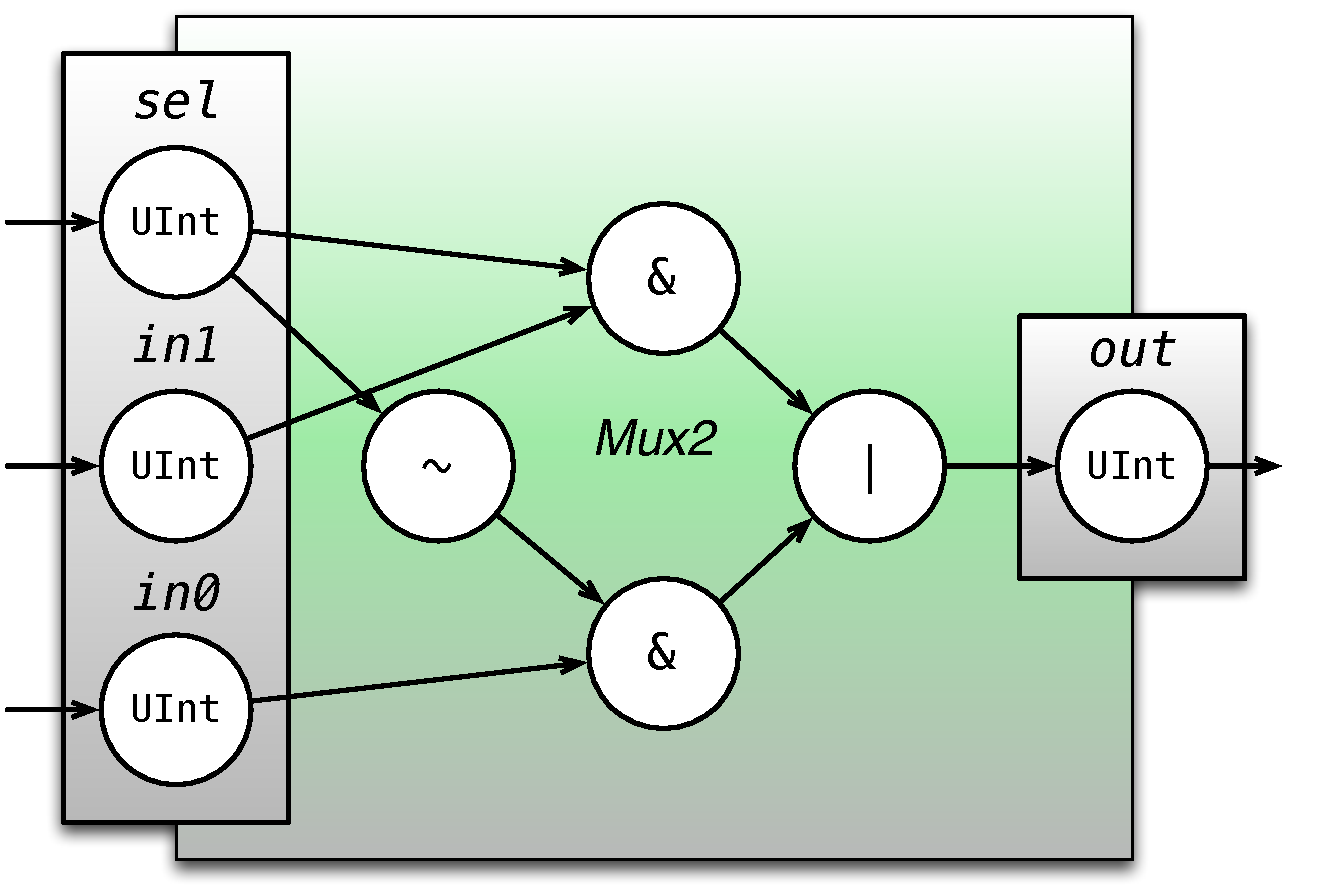
\includegraphics[width=0.9\textwidth]{figs/mux2-component.pdf} 
\end{center}

\end{columns}

\end{frame}

\begin{frame}{Chisel Workflow}
\begin{center}
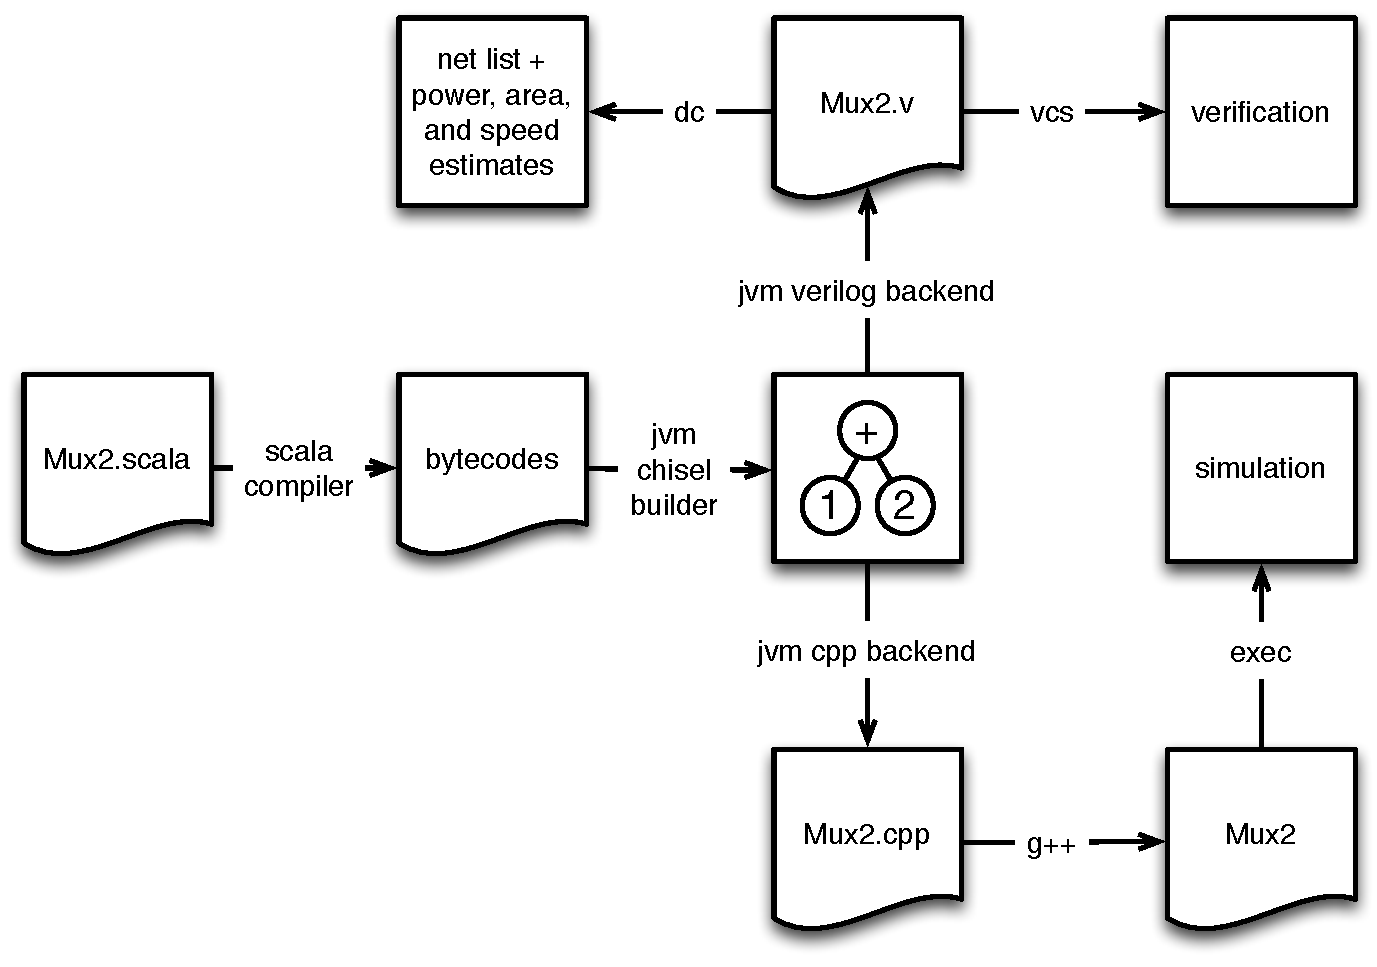
\includegraphics[height=0.9\textheight]{../bootcamp/figs/chisel-workflow.pdf}
\end{center}
\end{frame}



\begin{frame}[fragile]{State Elements}

\begin{scala}
Reg(data = in)
\end{scala}

\begin{center}
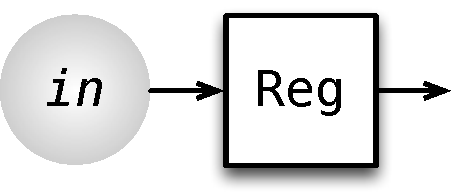
\includegraphics[width=0.9\textwidth]{figs/reg-in.pdf} 
\end{center}

\end{frame}

\begin{frame}[fragile]{Rising Edge}

\begin{scala}
def risingEdge(x: Bool) = x && !Reg(data = x)
\end{scala}

\begin{center}
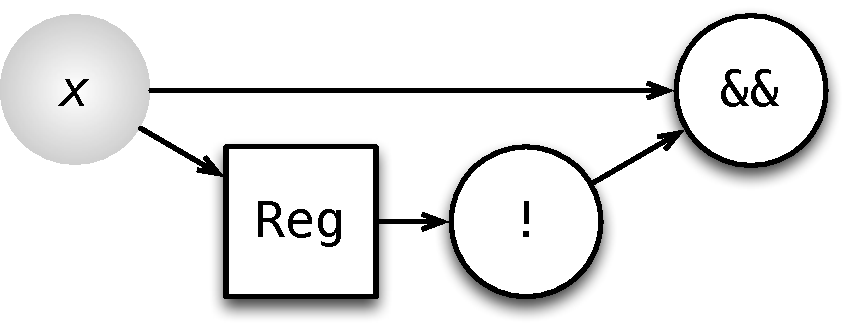
\includegraphics[width=0.9\textwidth]{figs/rising-edge.pdf} 
\end{center}

\end{frame}

\begin{frame}[fragile]{Counter}

\begin{columns}
\column{0.6\textwidth}

\begin{scala}
def counter(max: UInt) = {
  val x = Reg(reset = UInt(0, max.getWidth))
  x := Mux(x == max, UInt(0), x + UInt(1))
  x
}
\end{scala}

\column{0.3\textwidth}

\begin{center}
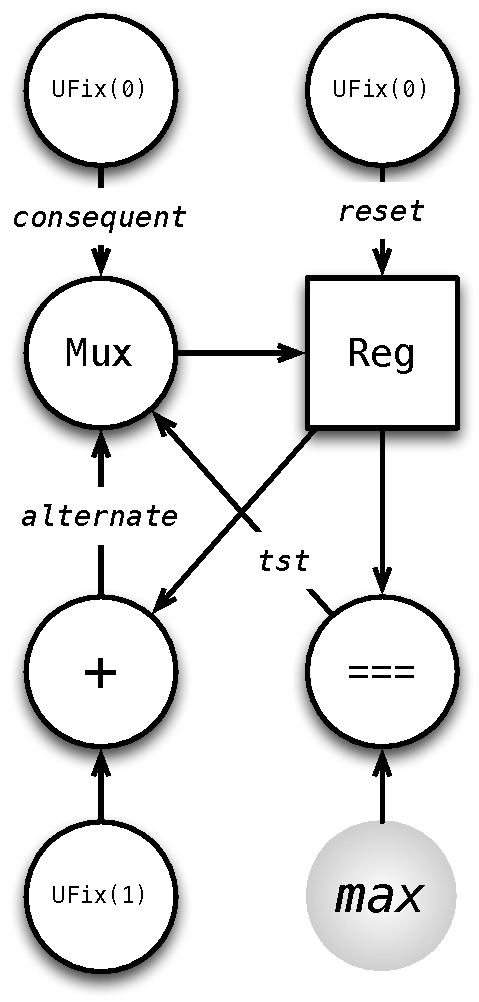
\includegraphics[height=0.9\textheight]{figs/counter.pdf} 
\end{center}

\end{columns}

\end{frame}

\begin{frame}[fragile]{Sequential Circuits}

\begin{scala}
// Produce pulse every n cycles.
def pulse(n: UInt) = counter(n - UInt(1)) === UInt(0)
\end{scala}

\begin{scala}
// Flip internal state when input true.
def toggle(p: Bool) = {
  val x = Reg(reset = Bool(false))
  x := Mux(p, !x, x)
  x
}
\end{scala}

\begin{scala}
// Square wave where each half cycle has given period.
def squareWave(period: UInt) = toggle(pulse(period))
\end{scala}

\end{frame}

\end{document}
